\documentclass{report}
\usepackage[T1]{fontenc} % Fontes T1
\usepackage[utf8]{inputenc} % Input UTF8
\usepackage[backend=biber, style=ieee]{biblatex} % para usar bibliografia
\usepackage{csquotes}
\usepackage[portuguese]{babel} %Usar língua portuguesa
\usepackage{blindtext} % Gerar texto automaticamente
\usepackage[printonlyused]{acronym}
\usepackage{hyperref} % para autoref
\usepackage{graphicx}
\usepackage{indentfirst}
\usepackage{float}
\addbibresource{bibliografia.bib}


\begin{document}
%%
% Definições
%
\def\titulo{Eletroencefalografia e Eye Tracking }
\def\data{08 de novembro de 2023}
\def\autores{Dinis Bernardo, Joana Santiago}
\def\autorescontactos{(120420) dinis.mvb@ua.pt, (119705) joanassantiago@ua.pt}
\def\versao{Versão 1}
\def\departamento{Dept. de Eletrónica, Telecomunicações e Informática}
\def\empresa{Universidade de Aveiro}
\def\logotipo{ua.pdf}
\def\repositorio{Repositório no github: infor2023-ap-g19}
%
%%%%%% CAPA %%%%%%
%
\begin{titlepage}

\begin{center}
%
\vspace*{50mm}
%
{\Huge \titulo}\\ 
%
\vspace{10mm}
%
{\Large \empresa}\\
%
\vspace{10mm}
%
{\LARGE \autores}\\ 
%
\vspace{30mm}
%
\begin{figure}[h]
\center
\includegraphics{\logotipo}
\end{figure}
%
\vspace{20mm}
\end{center}
%
\begin{flushright}
\versao
\end{flushright}
\end{titlepage}

%%  Página de Título %%
\title{%
{\Huge\textbf{\titulo}}\\
{\Large \departamento\\ \empresa}
}
%
\author{%
    \autores \\
    \autorescontactos \\
    \repositorio
}
%
\date{\today}
%
\maketitle

\pagenumbering{roman}

%%%%%% RESUMO %%%%%%
\begin{abstract}

A \ac{eeg} é uma técnica que regista a atividade existente no cérebro por meio de elétrodos colocados na cabeça, em que estes captam os sinais elétricos gerados pelas sinopses. O \ac{eeg} é bastante utilizado para uso médico, para pesquisas cientificas e já começa a ser utilizado para jogos, como Elden Ring, Trackmania, Minecraft, entre outros.

Já o \ac{et} é uma técnica que monitoriza e regista os movimentos dos olhos de uma pessoa, através do uso de dispositivos que capturam os movimentos oculares, como câmaras infravermelhas. O \ac{et} é utilizado em diversas áreas como a pesquisa de mercado, psicologia, comportamento visual, e até pode ser usado por empresas para entenderam o processo dos seus trabalhadores. Tal como a \ac{eeg}, o \ac{et} também já começa a aparecer em diversos jogos.

A \ac{eeg} e o \ac{et} são duas tecnologias muito inovadoras, e a combinação destas duas ferramentas é bastante útil em pesquisas que procuram entender como o cérebro e os olhos interagem em diferentes situações, quando aquilo que vemos esta ligado ás ondas cerebrais que são produzidas. Estas duas tecnologias também ajudam bastante a incluir pessoas que tenham problemas de saúde a sentirem-se incluídos na comunidade de jogadores, além disso oferece uma experiência fora do normal para todos os jogadores. 
\end{abstract}

%%%%%% Agradecimentos %%%%%%
% Segundo glisc deveria aparecer após conclusão...
%\renewcommand{\abstractname}{Agradecimentos}
%\begin{abstract}
%Eventuais agradecimentos.
%Comentar bloco caso não existam agradecimentos a fazer.
%\end{abstract}

\renewcommand{\contentsname}{Índice}
\tableofcontents
 \listoftables     % descomentar se necessário
 \listoffigures    % descomentar se necessário


%%%%%%%%%%%%%%%%%%%%%%%%%%%%%%%
\clearpage
\pagenumbering{arabic}

%%%%%%%%%%%%%%%%%%%%%%%%%%%%%%%%
\chapter{Introdução}
\label{chap.introducao}

Este relatório tem como principal objetivo aprofundar o tema do uso de Eletroencefalografia (\ac{eeg}) junto da tecnologia de Eye Tracking (\ac{et})  para usos tanto medicinais como de entretenimento. \ac{eeg} é um método usado para registar a atividade cerebral de uma maneira não invasiva, já a tecnologia \ac{et} consegue medir a posição exata para onde o utilizador está a olhar tanto como os seus movimentos oculares. Assim, podem ser criadas interfaces de utilização através apenas do cérebro e olhos do utilizador.

O objetivo deste estudo é entender como é que estas tecnologias podem beneficiar áreas como a da saúde, como ajudar pessoas que sejam incapazes de utilizar meios convencionais para usar um computador fazê-lo na mesma, e também como é que estas servirão para a criação de novos meios de entretenimento.
Este documento está dividido em quatro capítulos. Depois desta introdução, no \autoref{chap.EEG} é apresentada o conceito da \ac{eeg}, os seus princípios de avaliação, o uso médico e os casos da sua utilização por necessidade,  no \autoref{chap.ET} é apresentada o conceito do \ac{et} e as suas aplicações, no \autoref{chap.EEGandET} é apresentada as aplicações da \ac{eeg} juntamente do \ac{et} nos videojogos e a vitalização desta tecnologia nos media, sendo estes discutidos no \autoref{chap.analise}. Finalmente, no \autoref{chap.conclusao} são apresentadas
as conclusões do trabalho.

\chapter{Eletroencefalografia}
\label{chap.EEG}


\section{Conceito}
A \ac{eeg} é um método de monitoria eletrofisiológica utilizada para registar a atividade elétrica do cérebro, envolvendo a análise da atividade de bilhões de neurónios ao medir o potencial elétrico na superfície do escalpo.\cite{Eletroencefalografia} Os elétrodos, posicionados no couro cabeludo, captam o sinal de atividade interna, percorrendo correntes elétricas através de diversas camadas cerebrais, do líquido cefalorraquidiano e do crânio.

O sinal registado tem origem no fluxo de iões pelo líquido extra-celular, atuando como um condutor elétrico quase ideal. Esse fenómeno está associado à atividade síncrona de vários neurónios, alinhados na mesma direção. A captação desses potenciais na superfície do escalpo é realizada por um voltímetro posicionado entre dois elétrodos, conforme esquematizado na Figura 2.1.

É relevante observar que o sinal da \ac{eeg} não especifica se a atividade neuronal foi de emissão ou receção, devido à impossibilidade de determinar com precisão em qual região do dendrito (parte dos neurónios que recebe informações de outros neurónios) ocorreu a sinapse. Essa técnica destaca-se por sua precisão temporal na ordem de segundos e sensibilidade espacial considerável, decorrente da correlação dos dados provenientes de cada elétrodo.

\section{Princípios de avaliação}

O padrão de oscilação no \ac{eeg} sofre alterações na frequência e amplitude, dependendo da atividade cerebral realizada. Uma maior amplitude está associada a menor frequência, e vice-versa. 

A amplitude de uma onda refere-se à magnitude máxima da oscilação ou variação em torno de um ponto de referência em uma forma de onda. Em termos mais simples, é a altura máxima (ou profundidade mínima, se a onda for uma onda sinodal) da onda medida a partir de sua linha de base. 
A partir de uma \ac{eeg} podemos distinguir essencialmente cinco tipos de ondas cerebrais:
\begin{itemize}
    \item As \textbf{ondas Delta}, que estão associadas ao sono profundo e que desempenham um papel crucial na regeneração e restauração do corpo durante o repouso, com 0,5 - 3 oscilações por segundo \ref{fig:2.2};
    \item As \textbf{ondas Teta}, relacionadas com momentos de relaxamento, indicam estados de consciência menos alerta, com 4 - 7 oscilações por segundo \ref{fig:2.3};
    \item As \textbf{ondas Alfa}, aparecem quando temos sono, e estão associadas a estados de mente relaxada, e estão na zona das 08 - 15 oscilações por segundo \ref{fig:2.4};
    \item As \textbf{ondas Beta}, quando estamos conscientes e com a mente pouco ativa e são observadas durante períodos de ansiedade leve, entre 16 - 31 oscilações por segundo \ref{fig:2.5}; 
    \item As \textbf{ondas Gama}, acima de 32 oscilações por segundo que aparecem quando se está a utilizar dois ou mais sentidos (visão, tato) \ref{fig:2.6}. 
\end{itemize}

Estas ondas cerebrais não só refletem atividades mentais específicas, mas também podem indicar problemas que uma pessoa possa ter, como por exemplo, mudanças nas ondas Delta podem indicar distúrbios no sono, enquanto alterações nas ondas Alfa podem estar relacionadas a condições de ansiedade e stresse. A análise das ondas pode ser clinicamente relevante. Pacientes com distúrbio do sono, a identificação de padrões específicos de ondas Delta pode orientar estratégias de tratamento. Já os que tem transtornos de ansiedade, a análise das ondas Alfa fornece informações sobre o estado emocional.

Podemos assim perceber que a \ac{eeg} não apenas oferece uma visão das atividades cerebrais, mas também desempenha um papel crucial na compreensão e no tratamento de condições clínicas diversas. 
\section{Uso médico}
A tecnologia de \ac{eeg} desempenha um papel essencial no domínio da medicina, sendo concebida não apenas para o diagnostico de deficiências mentais/cerebrais, mas também para diversos usos medicinais. 
Por exemplo, o caso de pacientes com epilepsia, podem ser feitas \ac{eeg} de rotina para determinar se ainda existe necessidade de o paciente continuar a tomar o medicamento anti-epilético, oferecendo uma abordagem monitorada e personalizada para o tratamento dessa condição neurológica.
Apresenta-se aqui uma lista das circunstâncias clínicas em que é mais comum o uso de \ac{eeg}:
\begin{enumerate}
    \item Para servir como complemento do teste de morte cerebral;
    \item Para diagnosticar pacientes em coma;
    \item Para ser compreender se um paciente é epilético ou possui outro tipo de transtorno neuronal...
\end{enumerate}

Para uma compreensão mais detalhada, está presente a seguir uma tabela com a correspondência entre a banda da frequência da \ac{eeg} com o possível diagnóstico:
\clearpage
\begin{table}[htb]
    \centering  
    \begin{tabular}{|p{0.25\linewidth}|p{0.25\linewidth}|p{0.25\linewidth}|p{0.25\linewidth}|} 
        \hline
         Banda&  Frequência em \ac{hz}&  Atividade cerebral prevista& Possível estado patológico\\
         \hline
         Delta&  < 4 &  Sono& Lesões sub-corticais ligeiras\\
         \hline
         Teta&  4 – 7 &  Inatividade& Lesões sub-corticais focais\\
         \hline
         Alfa&  8 – 15 &  Mente relaxada& Estado de coma \\
         \hline
         Beta&  16 – 31 &  Mente ativa, foco, ansiedade leve& Possíveis transtornos relacionados com ansiedade crónica\\
         \hline
         Gama&  32 + &  Sensações tácteis, uso de vários sentidos simultaneamente& Declínio cognitivo\\
         \hline
    \end{tabular}
    \caption{Tabela adaptada da tabela presente na \href{https://pt.wikipedia.org/wiki/Eletroencefalografia}{Wikipedia da \ac{eeg}} }
    \label{tab:my_label}
\end{table}

Claro que ainda não pode ser feito um diagnóstico apenas com as \ac{eeg}, mas junto com outros procedimentos, são uma poderosa ajuda, obtendo assim uma avaliação mais completa das condições cerebrais. Existem também outras tecnologias parecidas para serem feitas análises ao cérebro, mas nenhuma é tão pouco invasiva como a \ac{eeg}.
Existem também outros usos a não ser medicinais para a \ac{eeg} como a criação de jogos interativos para aprendizagem e demonstração das capacidades da tecnologia. \cite{BrainSupport}

\section{Casos da sua utilização por necessidade}
Com o recente e acelerado desenvolvimento do uso prático da \ac{eeg}, uns cientistas na Suíça começaram o desenvolvimento de uma cadeira de rodas para pessoas completamente paralisadas, que fará uso exclusivo da tecnologia de \ac{eeg} para controlar uma cadeira de rodas, não sendo necessário andar sempre alguém junto destas pessoas. Para testes e protótipos iniciais, os cientistas criaram um videojogo de corridas em que o carro é controlado quando o utilizador tentar mexer as suas diferentes partes do corpo, ou pelo menos imaginá-lo. O que surpreendeu os cientistas foi a facilidade com que os utilizadores, todos sem capacidades motoras do pescoço para baixo, foram capazes de jogar o jogo. \cite{WralNews}



\newpage
%%%%%%%%%%%    FIGURAS     %%%%%%%%%%%%%%

\begin{figure}
    \centering
    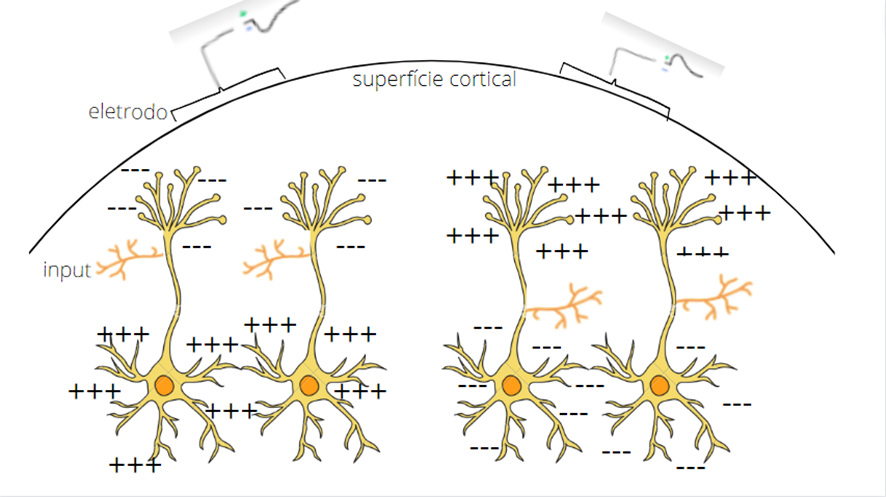
\includegraphics[width=0.5\linewidth]{Figura_1_–_Neurônios_em_atividade_síncrona_e_orientada_até_o_eletrodo.png}
    \caption{Funcionamento dos elétrodos usados na \ac{eeg}.}
    \label{fig:2.1}
\end{figure}

\begin{figure}
    \centering
    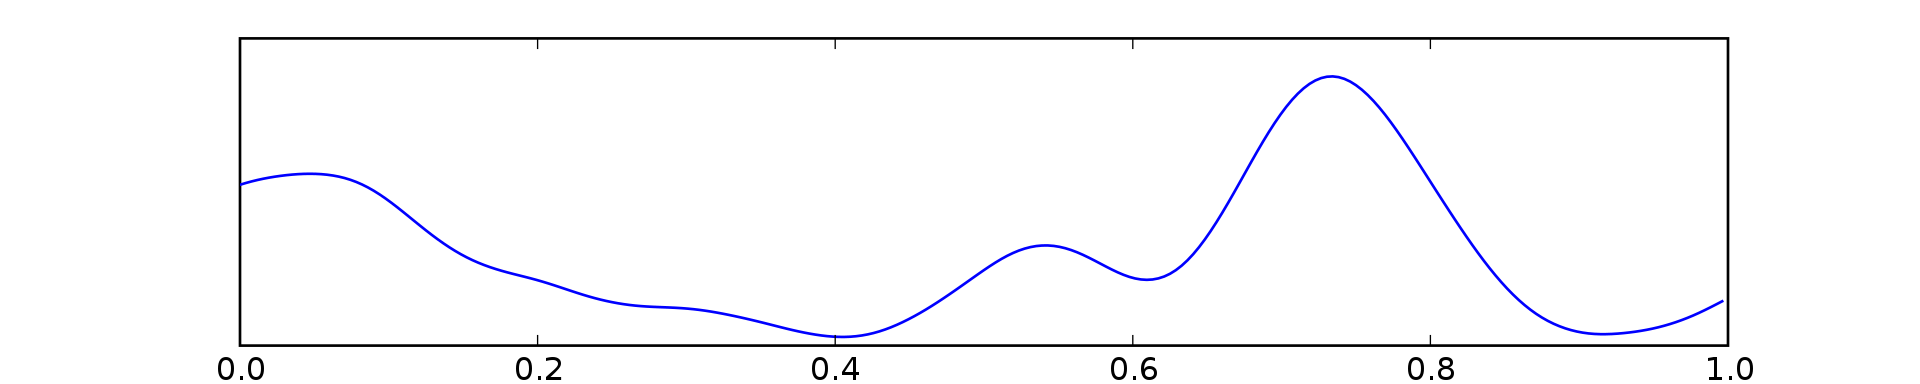
\includegraphics[width=0.7\linewidth]{Eeg_delta.svg.png}
    \caption{Ondas Delta}
    \label{fig:2.2}
\end{figure}

\begin{figure}
    \centering
    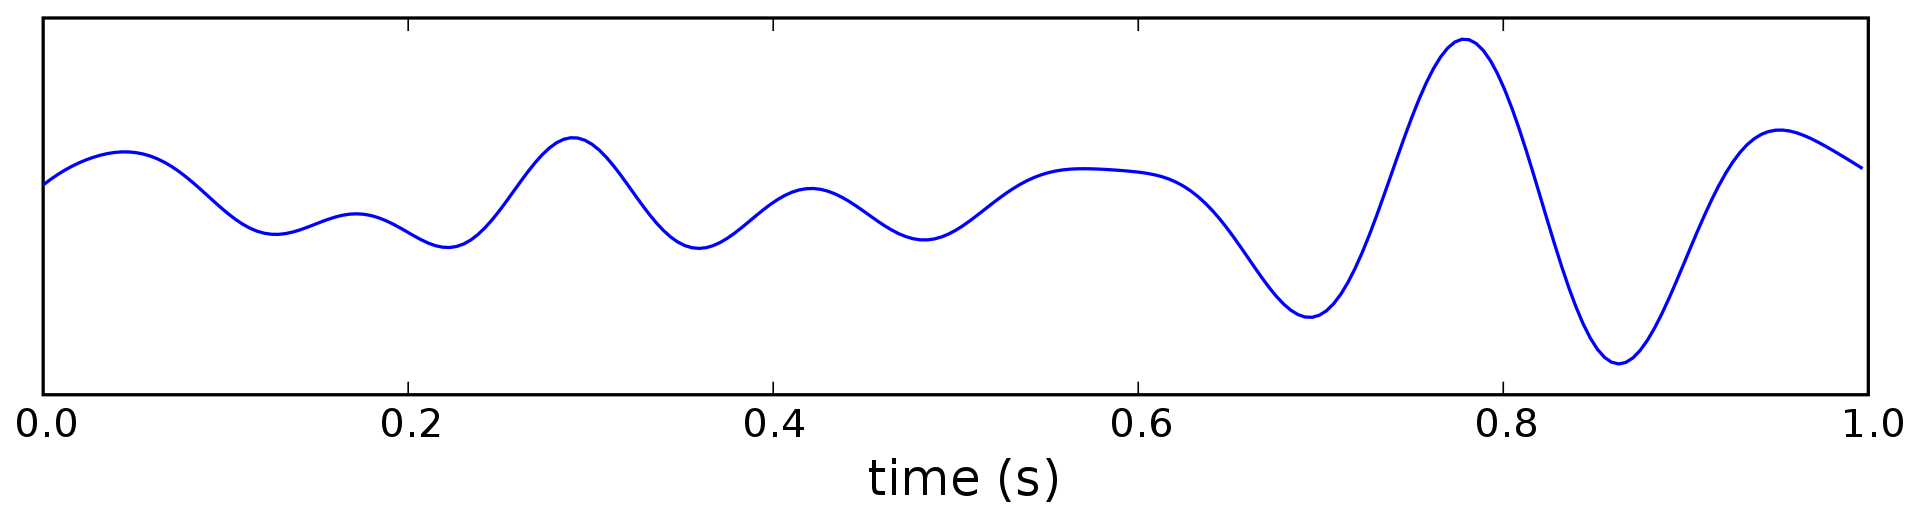
\includegraphics[width=0.6\linewidth]{Eeg_theta.svg.png}
    \caption{Ondas Teta}
    \label{fig:2.3}
\end{figure}

\begin{figure}
    \centering
    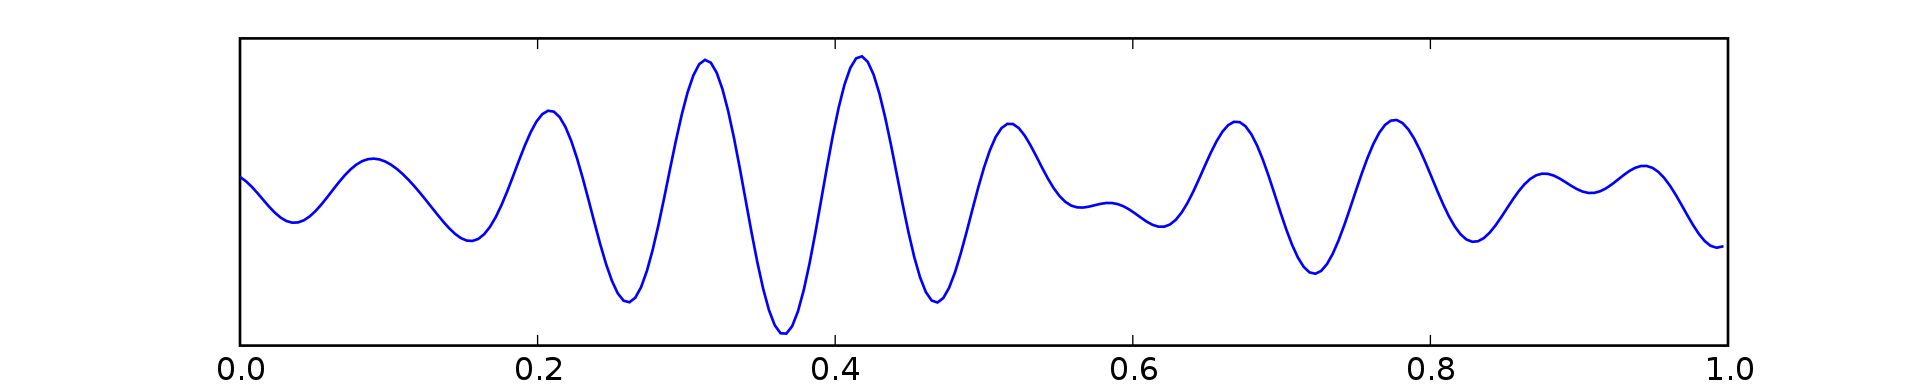
\includegraphics[width=0.7\linewidth]{Eeg_alpha.svg.png}
    \caption{Ondas Alfa}
    \label{fig:2.4}
\end{figure}

\begin{figure}
    \centering
    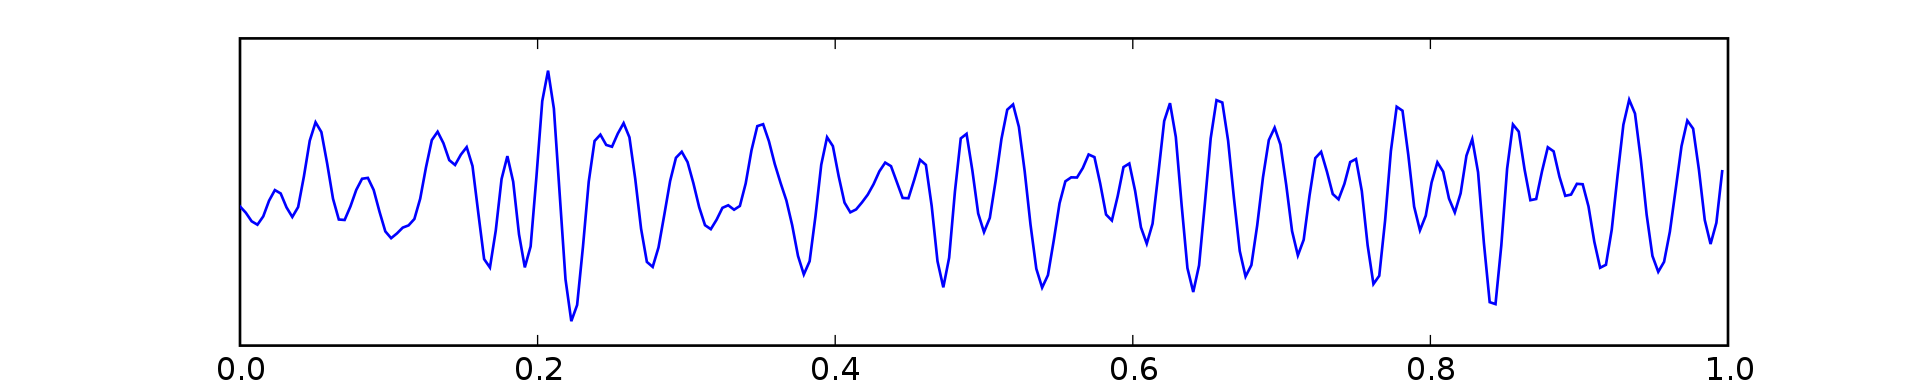
\includegraphics[width=0.7\linewidth]{Eeg_beta.svg.png}
    \caption{Ondas Beta}
    \label{fig:2.5}
\end{figure}

\begin{figure}
    \centering
    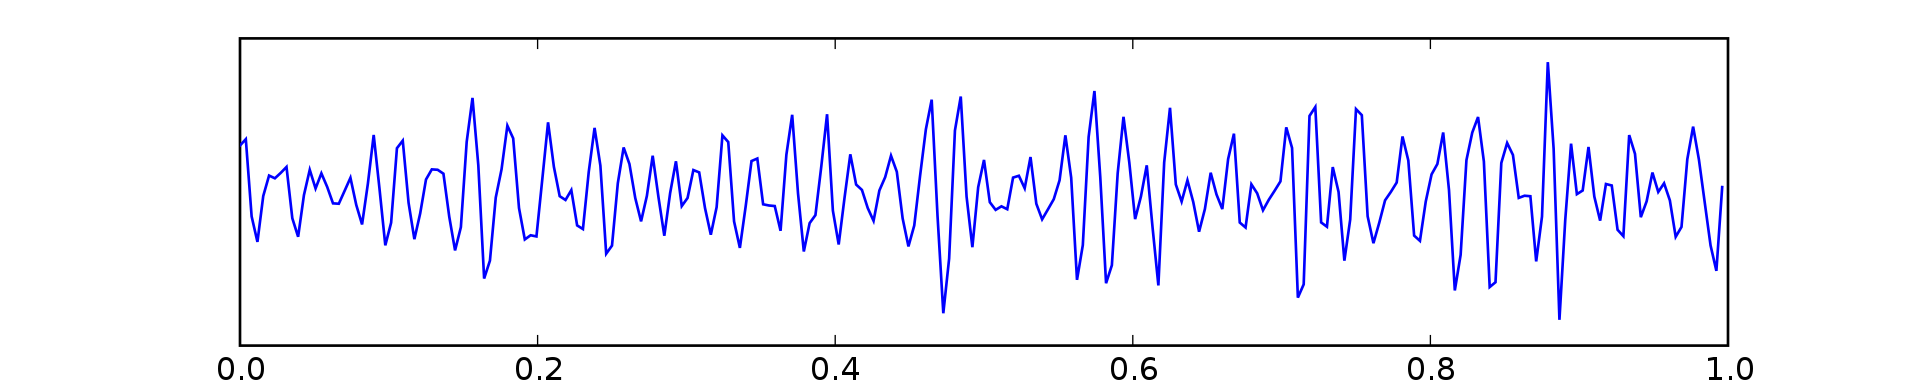
\includegraphics[width=0.7\linewidth]{Eeg_gamma.svg.png}
    \caption{Ondas Gama}
    \label{fig:2.6}
\end{figure}

%%%%%%%%%%%%%%%%%%%%%%%%%%%%%%%%%%%%%%%%%%


\chapter{Eye Tracking}
\label{chap.ET}

\section{Conceito}
O \ac{et}, constitui uma tecnologia avançada dedicada à observação e registo minucioso dos movimentos oculares de um individuo \cite{EyeTracking}. O seu principal objetivo é captar a direção do olhar, analisar os padrões de movimento ocular e na compreensão de como os olhos reagem aos estímulos visuais. Por meio de sensores especializados, o \ac{et} possibilita a coleta de dados precisos sobre a posição e movimentos dos olhos.
Existem 4 maneiras principais de ser feito o \ac{et}, sendo estas:
\begin{enumerate}
    \item \textbf{\ac{et} "agarrado" aos olhos}, em que o utilizador tem de ter uma lente ou outro aparelho que fisicamente regista os movimentos oculares. Este método, embora barato e fácil de aplicar, é o com menor precisão dos apresentados.;
    \item \textbf{\ac{et} através de uma lente}, em que o utilizador tem de ter um aparelho, como o da figura \ref{fig:3.1}, que para além de caro, é pesado, o que dificulta usos de \ac{et} por sessões prolongadas. Este método é o com mais precisão dos apresentados.;
    \item \textbf{\ac{et} através de medições de potenciais elétricos}, que seriam colocados ao redor dos olhos e detetam    a localização da íris e funcionariam mesmo com os olhos fechados ou sem luz. A desvantagem deste método é que é comum haver interferências que dão falsos positivos do movimento ocular.
    \item \textbf{\ac{et} através de uma câmara em frente ao utilizador}, este é o método mais comum e consiste apenas numa câmara que se encontra por cima do que se pretenda que o utilizador observe, e através de filmagens em tempo real dos olhos do utilizador consegue determinar para onde está a olhar, é muito pouco invasivo e distrativo, mas depende fortemente da qualidade da câmara utilizada.
\end{enumerate}

Irá ser, a partir de agora, ser feita referência ao quarto método sempre que falarmos de \ac{et}, visto que é o mais prático e também o mais utilizado.

\section{Aplicações do Eye Tracking}
\begin{itemize}
    \item \textbf{Interfaces de Interatividade Humano-Computador:}

    
        \begin{itemize}
            \item Esta tecnologia é muito usada em conjunto com computadores para criar interfaces de interação humano-computador. A sua capacidade de rastrear o olhar permite que as interfaces adaptam-se ás ações visuais do usuário, proporcionando uma interação mais intuitiva e eficiente.
        \end{itemize}
    \end{itemize}
    
\begin{itemize}
    \item \textbf{Psicologia e Compreensão Comportamental:}

        \begin{itemize}
        \item Pode ser usado na psicologia, com finais de compreensão dos comportamentos humanos, como por exemplo na figura \ref{fig:3.2}, que representa os pontos para onde o típico humano olha quando está a ler algo, exemplificando como essa tecnologia contribui para a análise detalhada de padrões de leitura e comportamento visual. \cite{EEG&ET_reading}
        \end{itemize}
\end{itemize}
\begin{itemize}
    \item \textbf{Marketing:}

    \begin{itemize}
        \item    No campo de marketing, o \ac{et} serve para observar como é que as diferentes audiências-alvo reagem e observam os anúncios que aparecem nos \textit{social media}, ajudando assim a criar estratégias de publicidade e design de conteúdo. \cite{ET_Pesquisas} \ref{fig:3.3}
    \end{itemize}
\end{itemize}
\begin{itemize}
    \item \textbf{Saúde:}    
        \begin{itemize}
        \item Com o estudo do comportamento visual, consegue-se obter informações muito importantes acerca do desenvolvimento, padrões de aprendizagem e sinais de doença, como por exemplo o Alzheimer, autismo, depressão, entre muitas outras.
    \end{itemize}
    
\end{itemize}
\begin{itemize}
    \item \textbf{Trabalho:}
    \begin{itemize}
        \item O \ac{et} também pode ser utilizado por empresas para entenderem os processos dos seus trabalhadores, e assim poderem identificar possíveis riscos de segurança, poupando assim muito tempo e melhorando a produtividade.
    \end{itemize}
\end{itemize}
\begin{itemize}
    \item \textbf{Adaptações de Software para Pessoas com Deficiências Motoras:}
    \begin{itemize}
        \item Para além de ser usada para estudos, pode também ser feitas adaptações de software para pessoas com deficiências motoras para que consigam usar os olhos como um rato num computador, por exemplo.
    \end{itemize}
\end{itemize}
\clearpage


%%%%%%%%%%%%  FIGURAS  %%%%%%%%%%%%%%%%%%%%%%%%%
\begin{figure}
    \centering
    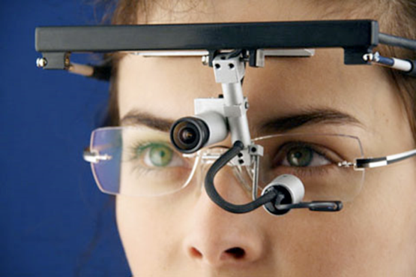
\includegraphics[width=0.75\linewidth]{20170731-eye-6.2.png}
    \caption{Aparelho de \ac{et}}
    \label{fig:3.1}
\end{figure}

\begin{figure}
    \centering
    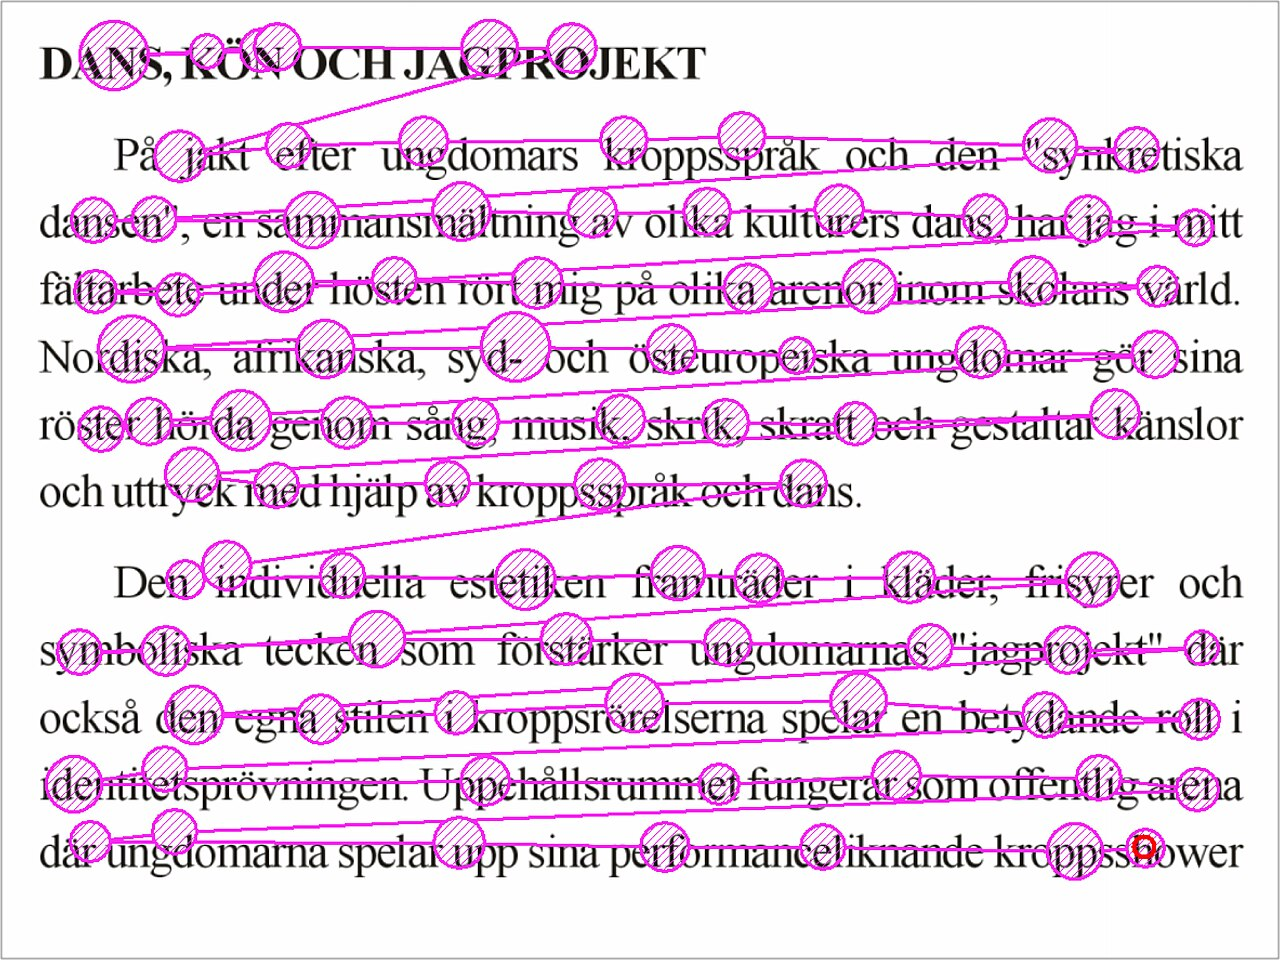
\includegraphics[width=0.75\linewidth]{Reading_Fixations_Saccades.jpg}
    \caption{Estudo feito que teve como objetivo entender como os olhos de um leitor se comportam}
    \label{fig:3.2}
\end{figure}

\begin{figure}
    \centering
    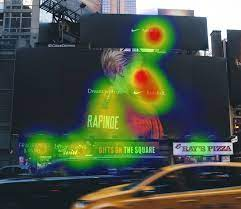
\includegraphics[width=0.75\linewidth]{download.jpeg}
    \caption{Mapa de calor que representa os locais que mais retém a atenção do público ao observar um anúncio na rua}
    \label{fig:3.3}
\end{figure}



%%%%%%%%%%%%%%%%%%%%%%%%%%%%%%%%%%%%%%%%%%%%%%%%%

\chapter{Eletroencefalografia junto da tecnologia de Eye Tracking}
\label{chap.EEGandET}

\section{Aplicações da Eletroencefalografia e Eye Tracking nos videojogos}

A combinação do \ac{eeg} e do \ac{et} tem diversas aplicações bastante interessantes e úteis nos jogos, que podem nos ajudar bastante a ter uma experiência única a que não estamos habituados. \cite{EEG&ET_VideoGames}
\begin{itemize}
    \item \textbf{Adaptação da Dificuldade do Jogo\textbf{:}}
    \begin{itemize}
        \item A análise da atividade cerebral pode avaliar o nível de atenção do jogador.
        \item Se o jogador não estiver a gostar do jogo, o sistema pode ajustar a dificuldade do jogo para que o jogador se entretenha mais.
    \end{itemize}
\end{itemize}
\begin{itemize}
    \item \textbf{Feedback Emocional em Tempo Real:}
        \begin{itemize}
            \item A \ac{eeg} pode ser utilizada para detetar emoções do jogador, como o tédio, a excitação ou a tristeza. Essa informação é usada para ajustar elementos do jogo, como a trilha sonora, iluminação e enredo, para melhorar a experiência do jogador.
        \end{itemize}
    \end{itemize}
\begin{itemize}
    \item \textbf{Controle por pensamento:}
        \begin{itemize}
            \item Visto que a \ac{eeg} permite a exploração do controle por pensamento, pode assim adicionar certos comandos através dos pensamentos do jogador, o que pode ser bastante útil para jogadores com modalidade reduzida.
        \end{itemize}
    \end{itemize}
\begin{itemize}
    \item \textbf{Análise da Atenção Visual:}
        \begin{itemize}
            \item O \ac{et}, neste caso, é utilizado para entender para onde o jogador está a olhar durante o jogo. Essa informação pode ser utilizada, por exemplo, para controlar a direção em que o personagem do jogo vai, ou até para otimizar a renderização gráfica na área em que o jogador esta a observar.
        \end{itemize}
    \end{itemize}
\begin{itemize}
    \item \textbf{Personalização da Narrativa:}
        \begin{itemize}
            \item Através das reações emocionais e níveis de engajamento, o jogo pode adaptar a narrativa ao que o jogador prefere e ajudar a determinar os elementos da história que mais lhe interessam.
        \end{itemize}
    \end{itemize}
\begin{itemize}
    \item \textbf{Avaliação da Experiência do Utilizador:}
        \begin{itemize}
            \item A combinação do \ac{eeg} e \ac{et} pode ser utilizada para avaliar a experiência do jogador em tempo real.
        \end{itemize}
        \begin{itemize}
            \item  Através da avaliação, os desenvolvedores dos jogos são capazes de perceber as áreas do jogo que são mais cativantes e as que precisam de melhorias.
        \end{itemize}
    \end{itemize}
\begin{itemize}
    \item \textbf{Prevenção de Fadiga:}
     \begin{itemize}
         \item A monitorização da atividade cerebral poderá ajudar a detetar problemas de fadiga, fazendo assim com que o jogo responda de maneira a reduzir a intensidade do estímulo ou sugerindo pausas para evitar a exaustão.

     \end{itemize}
     \item \textbf{Treino Mental:}
     \begin{itemize}
         \item Em conjunto com jogos, a \ac{eeg} pode ser utilizada para melhorar a concentração, a memória e capacidades.
     \end{itemize}
 \end{itemize}

Uma equipa da universidade de Ben-Gurion no Israel, propôs serem usadas estas tecnologias para aumentar a taxa de envolvimento de um jogador com um videojogo \cite{DDA}, pois existem vários aspetos que o podem irritar e fazer com que não queira continuar a jogar,como oponentes demasiado fortes, que são um fator desmotivante, ou pelo contrário, oponentes demasiado fracos, que tornam a experiência repetitiva e aborrecida sem necessidade de pensamento estratégico. Para isso, através da mistura entre \ac{eeg} e \ac{et}, pode ser feita uma análise dos comportamentos do jogador e do seu estado mental enquanto está envolvido num jogo para que o jogo se modifique e altere a dificuldade ou outros aspetos e torne a experiência mais divertida e viciante. É sugerido pela equipa que esta alteração para o desfrutar do utilizador seja aplicada apenas quando necessário, pois uma utilização da mesma em demasia pode causar um vício ou dependência no jogo em alguns casos, devido aos níveis de dopamina se encontrarem sempre ao máximo, já que este seria um eventual "jogo perfeito" para o utilizador.

Após alguns testes, a maioria dos jogadores admitiu preferir jogar em ambientes regulados para si do que um jogo constantemente muito desafiante ou muito fácil.

\section{Viralização desta tecnologia nos media}
Estas tecnologias ainda não são muito usadas, mas já começam a surgir pessoas a criar conteúdo e a desenvolver maneiras criativas da sua utilização para lazer, como por exemplo na plataforma de vídeos em direto chamada \textit{Twitch},um canal com nome de \href{https://www.twitch.tv/perrikaryal}{Perrikaryal} , desenvolveu uma maneira de jogar videojogos multi-jogador com \ac{eeg}, \ac{et} e alguns giroscópios, começando criar conteúdo à volta disso e a ganhar alguma popularidade.
\paragraph{}
Esta \textit{live-streamer} canadense-britânica, que tirou um doutoramento em psicologia, que está a desenvolver um protótipo de \ac{eeg} com fins medicinais, achou que seria uma boa ideia tentar completar um videojogo conhecido como um dos mais difíceis de sempre (o \textit{Elden Ring}, da \textit{From Software}) com a ajuda do seu protótipo\cite{EldenRing}, e os resultados que obteve foram bastante positivos, pois podia usar as duas mãos para a movimentação do seu personagem e curá-lo, e usar as ondas lidas pela \ac{eeg} para lançar feitiços e atacar, milhares de pessoas estavam lá para a ver a completar o último nível de um dos jogos mais difíceis de sempre. 
Desde então,  ao acrescentar a tecnologia de \ac{et} e alguns giroscópios na sua cabeça está a aperfeiçoar a sua interface que a permite jogar exclusivamente com a sua mente, olhos e algumas vezes movendo a cabeça.
\paragraph{}
E como é que funciona? Através de alguns estudos, conseguiu concluir que certos pensamentos diferentes, como por exemplo pensar na palavra "Atacar" ou "Eliminar" criam frequências lidas pela \ac{eeg} muito semelhantes entre si mas muito distintas de outros conceitos como "Curar" ou "Salvar". Através disto, associou cada uma das ações dos jogos que joga a certos pensamentos. Para mirar as armas e direcionar o personagem, faz uso do \ac{et} usando não só os movimentos oculares mas também consegue colocar alguns inputs no seu piscar de olhos e até mesmo olhar abaixo ou acima do monitor onde joga. Para finalizar e corrigir alguns eventuais erros que possam ocorrer, usa uns giroscópios junto à sua cabeça, que podem anular ações não entendidas assim como ajudar com a direção ocular.
\paragraph{}
Ao viralizar desta maneira, mais e mais pessoas começaram a querer experimentar em primeira mão este tipo de maneira de jogar, que para alguns até parece magia. E, dado isto, começa a surgir um muito maior fluxo de dinheiro para esta área, o que não só ajuda no seu desenvolvimento, mas também abre o mercado e torna estas tecnologias mais acessíveis para todos.

\chapter{Resultados}
\label{chap.resultados}

Os resultados em cada projeto realizado com a tecnologia de  \ac{eeg} e  \ac{et} são diferentes, visto que cada um é realizado por pessoas diferentes, com capacidades diferentes. Como referido anteriormente, a \textit{live-streamer} Perrikaryal, utiliza estas duas ferramentas para jogar alguns jogos, no entanto, e como era de esperar, a jogabilidade e a experiência do utilizador é completamente distinta do que sem a utilização destas duas tecnologias. 

Num jogo mais simples, Trackmania, jogo de corrida de carros, em que só são utilizados 4 comandos, com um objetivo mais direto, chegar a meta, o utilizador facilmente consegue estabelecer a relação entre o que quer que o carro faça e o que o carro realmente faz, e para isso utiliza movimentos de inclinação da sua cabeça para ajudar a visualizar o movimento pretendido, assim o jogador consegue experienciar o jogo de forma mais semelhante caso fosse utilizado um teclado.

Num segundo caso, o jogo Minecraft, jogo de construção e exploração num mundo infinito com o objetivo de sobrevivência para no final matar o monstro mais forte, torna-se muito mais desafiador e complexo, visto que neste jogo são precisos 6 comandos em vez de 4. Neste caso a \textit{live-streamer} primeiramente calibrou o seu programa de modo a guardar os seus estímulos, por exemplo, quando imaginava que partia um bloco o programa ativava um botão do comando. Foi um processo bastante demorado e trabalhoso, já que tinha de configurar muito bem o programa.
\chapter{Análise}
\label{chap.analise}
Com os resultados que se obteve, podemos analisar e perceber que, projetos com a utilização da \ac{eeg} e do \ac{et} são diferentes, devido ás diferenças individuais entre as pessoas que os realizam, destacando assim a influência das capacidades individuais na eficácia dessas tecnologias, bem como os jogos serem diferentes entre si, ou a finalidade destas ferramentas serem distintas.

Nos resultados em cima utiliza-se o exemplo do jogo Trackmania, que destaca que neste caso a relação entre os comandos e as ações do jogo é mais direta, facilitando assim a experiência do usuário. O outro exemplo de jogo foi o Minecraft, um jogo mais complexo, em que é destacado o desafio adicional de calibrar o programa para guardar estímulos cerebrais específicos a ações do jogo, salientando os desafios técnicos e a necessidade de uma configuração precisa para garantir que as tecnologias captem os estímulos desejados de forma eficaz. Isso ressalta as complexidades envolvidas na integração dessas tecnologias em jogos mais complicados.

 De acordo com o que está referido anteriormente, e tendo em conta a complexidade e dificuldade destes projetos, podemos afirmar que para objetivos menos simples, ou casos de uso com muitos comandos de ação, a experiência do utilizador é bastante diferente do ambiente que é sem a utilização destas ferramentas, contudo e tendo em conta ao nível de complexidade que envolve, os resultados obtidos foram bastante satisfatórios, uma vez quem, por muito que são as experiências, o sistema conseguiu alcançar o seu objetivo, e os utilizadores não ficaram insatisfeitos. 
\chapter{Conclusões}
\label{chap.conclusao}
Tanto a \ac{eeg} quanto o \ac{et} representam avanços significativos nas suas respetivas áreas de aplicação. A \ac{eeg}, uma técnica não invasiva para registar a atividade cerebral, e o \ac{et}, capaz de medir a posição do olhar e os movimentos oculares, oferecem a possibilidade de criar interfaces de usuário baseadas exclusivamente na interação entre o cérebro e os olhos do usuário.

O objetivo principal deste relatório foi explorar como essas tecnologias podem trazer benefícios significativos para a área de saúde, proporcionando meios de comunicação alternativos para aqueles que enfrentam limitações no uso de métodos convencionais para interagir com computadores. Além disso, investigou-se como essas tecnologias estão a transformar novas formas de entretenimento, especialmente no campo dos jogos.

Concluindo, este relatório destaca a importância e o potencial impacto positivo destas tecnologias. Estas não tem apenas o potencial de melhorar a qualidade de vida de indivíduos com limitações físicas, mas também promovem avanços inovadores no campo do entretenimento digital. A combinação de \ac{eeg} e \ac{et} oferece diversas oportunidades de pesquisa e desenvolvimento, indicando um futuro promissor para a integração dessas tecnologias em diversas áreas da sociedade.
\chapter*{Contribuições dos autores}
Cada autor contribui igualmente para o produto final do traballho, sendo justamente atribuido a nota de 50\% a cada um.

\vspace{10pt}
\textbf{Indicar a percentagem de contribuição de cada autor.}\\

\ac{db}, \ac{js}: 50\%, 50\%\\

%%%%%%%%%%%%%%%%%%%%%%%%%%%%%%%%%
\chapter*{Acrónimos}
\begin{acronym}
\acro{ua}[UA]{Universidade de Aveiro}
\acro{leci}[LECI]{Licenciatura em Engenharia de Computadores e Informática}
\acro{glisc}[GLISC]{Grey Literature International Steering Committee}
\acro{js}[JS]{Joana Santiago}
\acro{db}[DB]{Dinis Bernardo}
\acro{eeg}[EEG]{Eletroencefalografia}
\acro{et}[ET]{Eye Tracking}
\acro{hz}[HZ]{Hertz}
\end{acronym}


\printbibliography



\end{document}